% Options for packages loaded elsewhere
\PassOptionsToPackage{unicode}{hyperref}
\PassOptionsToPackage{hyphens}{url}
%
\documentclass[
]{article}
\usepackage{amsmath,amssymb}
\usepackage{lmodern}
\usepackage{ifxetex,ifluatex}
\ifnum 0\ifxetex 1\fi\ifluatex 1\fi=0 % if pdftex
  \usepackage[T1]{fontenc}
  \usepackage[utf8]{inputenc}
  \usepackage{textcomp} % provide euro and other symbols
\else % if luatex or xetex
  \usepackage{unicode-math}
  \defaultfontfeatures{Scale=MatchLowercase}
  \defaultfontfeatures[\rmfamily]{Ligatures=TeX,Scale=1}
\fi
% Use upquote if available, for straight quotes in verbatim environments
\IfFileExists{upquote.sty}{\usepackage{upquote}}{}
\IfFileExists{microtype.sty}{% use microtype if available
  \usepackage[]{microtype}
  \UseMicrotypeSet[protrusion]{basicmath} % disable protrusion for tt fonts
}{}
\makeatletter
\@ifundefined{KOMAClassName}{% if non-KOMA class
  \IfFileExists{parskip.sty}{%
    \usepackage{parskip}
  }{% else
    \setlength{\parindent}{0pt}
    \setlength{\parskip}{6pt plus 2pt minus 1pt}}
}{% if KOMA class
  \KOMAoptions{parskip=half}}
\makeatother
\usepackage{xcolor}
\IfFileExists{xurl.sty}{\usepackage{xurl}}{} % add URL line breaks if available
\IfFileExists{bookmark.sty}{\usepackage{bookmark}}{\usepackage{hyperref}}
\hypersetup{
  pdfauthor={Alaska Department of Health and Social Services Weekly COVID-19 and Influenva Update},
  hidelinks,
  pdfcreator={LaTeX via pandoc}}
\urlstyle{same} % disable monospaced font for URLs
\usepackage[margin=1in]{geometry}
\usepackage{graphicx}
\makeatletter
\def\maxwidth{\ifdim\Gin@nat@width>\linewidth\linewidth\else\Gin@nat@width\fi}
\def\maxheight{\ifdim\Gin@nat@height>\textheight\textheight\else\Gin@nat@height\fi}
\makeatother
% Scale images if necessary, so that they will not overflow the page
% margins by default, and it is still possible to overwrite the defaults
% using explicit options in \includegraphics[width, height, ...]{}
\setkeys{Gin}{width=\maxwidth,height=\maxheight,keepaspectratio}
% Set default figure placement to htbp
\makeatletter
\def\fps@figure{htbp}
\makeatother
\setlength{\emergencystretch}{3em} % prevent overfull lines
\providecommand{\tightlist}{%
  \setlength{\itemsep}{0pt}\setlength{\parskip}{0pt}}
\setcounter{secnumdepth}{-\maxdimen} % remove section numbering
\ifluatex
  \usepackage{selnolig}  % disable illegal ligatures
\fi

\title{
\includegraphics{C:/Users/ccross/Documents/Projects/COVID-19 Weekly Report R Markdown/logo.jpg}}
\author{Alaska Department of Health and Social Services Weekly COVID-19
and Influenva Update}
\date{March 27 -- April 2, 2022}

\begin{document}
\maketitle

~

~

\hypertarget{key-findings}{%
\subsubsection{Key Findings}\label{key-findings}}

\begin{itemize}
\item
  The incidence of COVID-19 remained as high or higher than it was
  before the Omicron wave across most parts of Alaska during the week of
  March 20--March 26, 2022, with mixed trajectories across boroughs and
  census areas. Case counts are no longer decreasing.
\item
  Appreciable levels of influenza transmission began occurring in
  mid-December but slowly declined over the last several weeks.
\item
  Other respiratory viruses are circulating in addition to SARS-CoV-2
  and influenza virus.
\item
  Beginning April 6, 2022, DHSS will be updating data on the Alaska
  COVID-19 Information Hub once a week, on Wednesdays, rather than the
  current three times weekly.
\end{itemize}

~

~

\hypertarget{covid-19}{%
\subsection{COVID-19}\label{covid-19}}

\hypertarget{covid-19-case-trends}{%
\subsubsection{COVID-19 Case Trends}\label{covid-19-case-trends}}

\begin{itemize}
\item
  COVID-19 transmission continues to occur widely throughout much of
  Alaska, with some evidence for an upwards trajectory. Cases and
  hospitalizations remain far below the peak of the Omicron wave.
\item
  2,461 cases were reported in Alaskans the week of March 6--March 12,
  however this includes a large number of older cases with delayed
  reporting, and the week-over-week increase in reported cases is not
  indicative of the true trend. The number of new cases statewide last
  week was similar to the number the week before.
\item
  The number of reported COVID-19 cases last week was lower in all five
  of the largest boroughs (Municipality of Anchorage, Matanuska-Susitna
  Borough, Fairbanks North Star Borough, Kenai Peninsula Borough, and
  the City and Borough of Juneau) compared to the previous week, though
  the declines were generally more modest than those observed in
  previous weeks.
\item
  The intensity of COVID-19 transmission varies between communities
  outside the largest boroughs. Trajectories are mixed, with COVID-19
  cases declining in many boroughs and census areas but increasing in
  others. Regardless, absolute levels of transmission remain high in
  many areas.
\item
  The Omicron variant accounts for effectively all SARS-CoV-2
  circulating in Alaska. An increasing proportion of COVID-19 cases in
  Alaska are caused by the BA.2 lineage (a sub-type of Omicron). Visit
  Alaska's SARS-CoV-2 Genomics Dashboard to learn more.
\item
  To learn more about COVID-19 cases, hospitalizations, and deaths due
  to COVID-19 in Alaska, visit the Cases Dashboard or the monthly
  report. The cases dashboard includes demographic information on cases
  and the monthly report includes demographic information on
  hospitalizations and deaths.
\end{itemize}

~

~

~

~

\begin{center}\includegraphics{COVID-19-Weekly-Report_files/figure-latex/Generate Table-1} \end{center}

\hypertarget{rates-based-on-20-observations-are-statistically-unreliable-and-should-be-used-with-caution.}{%
\subparagraph{*Rates based on \textless20 observations are statistically
unreliable and should be used with
caution.}\label{rates-based-on-20-observations-are-statistically-unreliable-and-should-be-used-with-caution.}}

\hypertarget{rates-based-on-6-observations-are-not-reported.}{%
\subparagraph{**Rates based on \textless6 observations are not
reported.}\label{rates-based-on-6-observations-are-not-reported.}}

\hypertarget{alert-levels-are-based-on-case-report-date.-the-case-rates-in-the-kusilvak-and-bethel-census-areas-are-artificially-elevated-this-past-week-due-to-processing-of-delayed-reports.}{%
\subparagraph{Alert levels are based on case report date. The case rates
in the Kusilvak and Bethel Census Areas are artificially elevated this
past week due to processing of delayed
reports.}\label{alert-levels-are-based-on-case-report-date.-the-case-rates-in-the-kusilvak-and-bethel-census-areas-are-artificially-elevated-this-past-week-due-to-processing-of-delayed-reports.}}

~

~

\hypertarget{covid-19-and-hospital-capacity}{%
\subsubsection{COVID-19 and Hospital
Capacity}\label{covid-19-and-hospital-capacity}}

\begin{itemize}
\item
  Hospital capacity remains limited. Large numbers of patients overall
  (not necessarily with COVID-19 or other respiratory viruses) relative
  to the number of available staff continue to create capacity
  challenges across the state, with some areas more affected than
  others.
\item
  Patient Care Strategies for Scare Resource Situations are currently
  not being utilized by any facility in Alaska. However, given the
  continued limited capacity of some facilities, the Crisis Care
  Committee continues to meet to monitor the situation and remains
  available to assist facilities and DHSS should the need arise.
\item
  As of March 14, 2022, there were 38 persons with COVID-19 in Alaska
  hospitals, accounting for 3.1\% of all hospitalized persons. Visit the
  Hospital Dashboard for more data.
\end{itemize}

~

~

~

~

\hypertarget{covid-19-and-vaccination}{%
\subsubsection{COVID-19 and
Vaccination}\label{covid-19-and-vaccination}}

\begin{itemize}
\item
  71.2\% of Alaska residents aged ≥5 years have received at least one
  dose of a COVID-19 vaccine. Among those who completed the primary
  vaccine series, 50.2\% of Alaska residents ≥18 years have received
  their booster. Learn more about COVID-19 vaccination coverage in
  Alaska on the Vaccine Dashboard. Learn more about COVID-19 vaccines.
\item
  Vaccines help protect against infection and against severe disease,
  especially when a person is up to date on vaccinations. During the
  4-week period from February 6, 2022--March 5, 2022, unvaccinated
  Alaskans were 7.3 times more likely to be hospitalized due to COVID-19
  than Alaskans who are up to date on COVID-19 vaccination (i.e.,
  completed the primary series and received a booster dose, if eligible)
  and 2.9 times more likely to be hospitalized due to COVID-19 than
  Alaskans who completed the primary vaccination series but are not up
  to date. These estimates are lagged by one week to partially account
  for the time it takes to document hospitalizations. (See the monthly
  report for more data and analysis through January.)
\end{itemize}

~

\hypertarget{unvaccinated-alaskans-are-7.3-times-more-likely-to-be-hospitalized-due-to-covid-19-than-alaskans-who-are-up-to-date-on-covid-19-vaccination-and-2.9-times-more-likely-to-be-hospitalized-due-to-covid-19-than-alaskans-who-completed-the-primary-vaccination-series-but-are-not-up-to-date.-in-order-to-more-easily-identify-changes-over-time-the-definition-of-up-to-date-as-of-january-8-2022-was-applied-to-data-from-all-time-points.-the-absolute-rates-of-hospitalization-especially-in-the-most-recent-4-week-period-highlighted-in-grey-are-likely-underestimates-because-of-covid-19-hospitalizations-that-have-not-yet-been-documented.-especially-when-rates-are-very-low-the-estimates-of-fold-differences-between-rates-may-be-imprecise.-fold-differences-are-not-calculated-if-one-of-the-rates-is-based-on-6-cases.}{%
\subparagraph{Unvaccinated Alaskans are 7.3 times more likely to be
hospitalized due to COVID-19 than Alaskans who are up to date on
COVID-19 vaccination and 2.9 times more likely to be hospitalized due to
COVID-19 than Alaskans who completed the primary vaccination series but
are not up to date. In order to more easily identify changes over time,
the definition of ``up to date'' as of January 8, 2022, was applied to
data from all time points. The absolute rates of hospitalization
especially in the most recent 4-week period highlighted in grey are
likely underestimates because of COVID-19 hospitalizations that have not
yet been documented. **Especially when rates are very low, the estimates
of fold-differences between rates may be imprecise. Fold-differences are
not calculated if one of the rates is based on \textless6
cases.}\label{unvaccinated-alaskans-are-7.3-times-more-likely-to-be-hospitalized-due-to-covid-19-than-alaskans-who-are-up-to-date-on-covid-19-vaccination-and-2.9-times-more-likely-to-be-hospitalized-due-to-covid-19-than-alaskans-who-completed-the-primary-vaccination-series-but-are-not-up-to-date.-in-order-to-more-easily-identify-changes-over-time-the-definition-of-up-to-date-as-of-january-8-2022-was-applied-to-data-from-all-time-points.-the-absolute-rates-of-hospitalization-especially-in-the-most-recent-4-week-period-highlighted-in-grey-are-likely-underestimates-because-of-covid-19-hospitalizations-that-have-not-yet-been-documented.-especially-when-rates-are-very-low-the-estimates-of-fold-differences-between-rates-may-be-imprecise.-fold-differences-are-not-calculated-if-one-of-the-rates-is-based-on-6-cases.}}

~

\begin{itemize}
\item
  Among Alaska residents aged ≥5 years from January 16, 2021--March 12,
  2022, 69,054 cases were documented in persons who had completed the
  primary series and were considered fully vaccinated. Among those
  vaccine-breakthrough cases, 515 hospitalizations and 180 deaths due to
  COVID-19 have been recorded. During that time, 98,276 cases have been
  documented in unvaccinated Alaskans aged ≥5 years, leading to 1,836
  hospitalizations and 642 deaths. All data are preliminary and subject
  to change.
\item
  During the Omicron wave, the incidence of COVID-19 cases in vaccinated
  persons has become more similar to the incidence in unvaccinated
  persons. This trend likely reflects multiple factors which may
  include: immunity wanes over time, cases in vaccinated persons may be
  more likely to be detected than cases in unvaccinated persons, and
  there may be increased infection-induced immunity especially among
  unvaccinated persons.
\end{itemize}

~

\hypertarget{in-order-to-more-easily-identify-changes-over-time-the-definition-of-up-to-date-as-of-january-8-2022-was-applied-to-data-from-all-time-points.-some-covid-19-cases-with-specimen-collection-in-the-immediate-past-week-indicated-by-the-grey-box-may-have-not-yet-been-reported-or-counted.}{%
\subparagraph{In order to more easily identify changes over time, the
definition of ``up to date'' as of January 8, 2022 was applied to data
from all time points. Some COVID-19 cases with specimen collection in
the immediate past week (indicated by the grey box) may have not yet
been reported or
counted.}\label{in-order-to-more-easily-identify-changes-over-time-the-definition-of-up-to-date-as-of-january-8-2022-was-applied-to-data-from-all-time-points.-some-covid-19-cases-with-specimen-collection-in-the-immediate-past-week-indicated-by-the-grey-box-may-have-not-yet-been-reported-or-counted.}}

~

~

~

\hypertarget{influenza-flu}{%
\subsection{Influenza (``Flu'')}\label{influenza-flu}}

\begin{itemize}
\item
  Reported influenza cases began increasing in Alaska in mid-December.
  The number of reported cases the week of March 27--April 2 remained
  similar to the number reported the previous week.
\item
  Right now, most influenza in Alaska is caused by influenza A. 24\% of
  Alaskans aged ≥10 years have been vaccinated against seasonal
  influenza. It is not too late to get vaccinated against influenza.
\item
  Learn more in the weekly Alaska Influenza Snapshot.
\end{itemize}

~

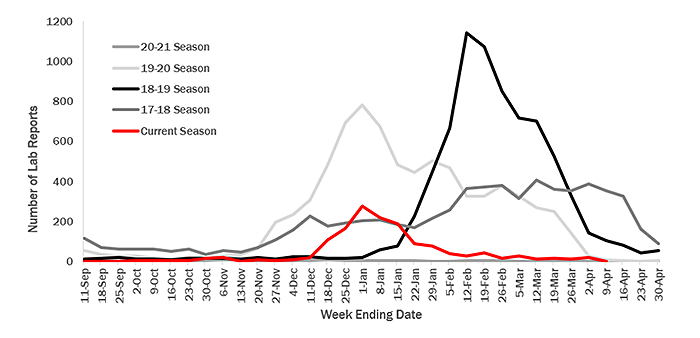
\includegraphics{/Users/ccross/Documents/Projects/COVID-19 Weekly Report R Markdown/6_original.png}

\hypertarget{positive-influenza-lab-reports-in-alaska-by-week-of-specimen-collection-for-the-2017-2018-influenza-season-through-present.-the-current-season-through-april-2-2022-is-shown-in-red.}{%
\subparagraph{Positive influenza lab reports in Alaska by week of
specimen collection for the 2017-2018 influenza season through present.
The current season through April 2, 2022 is shown in
red.}\label{positive-influenza-lab-reports-in-alaska-by-week-of-specimen-collection-for-the-2017-2018-influenza-season-through-present.-the-current-season-through-april-2-2022-is-shown-in-red.}}

~

~

~

\hypertarget{emergency-department-visits}{%
\subsection{Emergency Department
Visits}\label{emergency-department-visits}}

\hypertarget{visits-with-covid-like-or-influenza-like-illness}{%
\subsubsection*{Visits with COVID-like or Influenza-like
Illness}\label{visits-with-covid-like-or-influenza-like-illness}}

\begin{itemize}
\item
  Syndromic surveillance consists of analyzing data on symptoms and
  diagnoses among patients visiting emergency departments in Alaska. The
  main goal is to identify trends. Unlike case-based surveillance,
  syndromic surveillance does not depend on laboratory testing.
\item
  Influenza-like illness (ILI) is defined as having a fever and at least
  one other symptom, such cough or sore throat. Patients with a
  diagnosis of influenza are also included, regardless of symptoms.
\item
  COVID-like illness (CLI) encompasses a broader array of respiratory
  and other symptoms than influenza-like illness. This category also
  includes any patient with a diagnosis of COVID-19, regardless of
  symptoms.
\item
  Patients with a diagnosis of COVID-19 are excluded from the ILI
  category and, likewise, patients with a diagnosis of influenza are
  excluded from the CLI category. But a patient without a diagnosis for
  either could be included in both the CLI and ILI categories. CLI and
  ILI may be caused by respiratory viruses other than SARS-CoV-2 and
  influenza virus.
\item
  As the Delta variant wave waned in Alaska in late October and November
  2021, the percentage of emergency department patients with CLI
  declined. However, it increased in mid-December, reaching its peak in
  mid-January. Now, it is at a level lower than that observed in
  December before the Omicron wave. The percentage of emergency
  department patients with CLI the week of March 27--April 2 remained
  similar to the percentage recorded the prior week.
\item
  ILI levels increased in December but have since decreased from the
  late-December peak, remaining steady over the last few weeks.
\end{itemize}

~

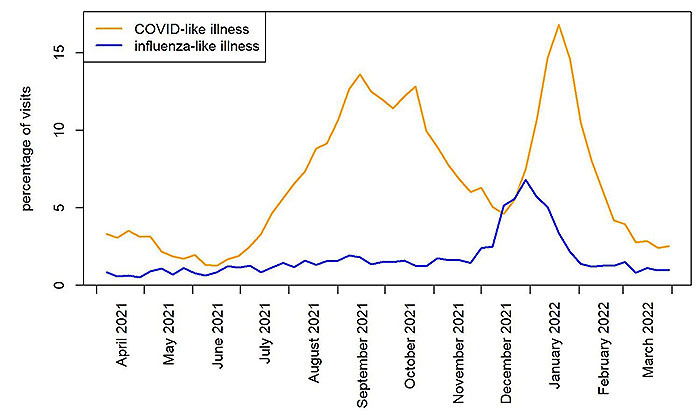
\includegraphics{/Users/ccross/Documents/Projects/COVID-19 Weekly Report R Markdown/7_original.jpg}

~

~

~

\hypertarget{new-updates}{%
\subsection{New Updates}\label{new-updates}}

\hypertarget{updates-to-protect-yourself-and-your-family}{%
\subsubsection*{Updates to protect yourself and your
family}\label{updates-to-protect-yourself-and-your-family}}

\begin{itemize}
\item
  Vaccine boosters: Everyone 12 or older should get a COVID-19 vaccine
  booster if it's been five months since receiving the Pfizer or Moderna
  vaccines or two months since receiving the Johnson \& Johnson vaccine.
  People over the age of 50 and some immunocompromised individuals may
  receive a second mRNA booster (Pfizer or Moderna) four months after
  their first booster dose. Additionally, people who have received the
  Johnson \& Johnson vaccine for both their primary dose and booster
  dose may receive a second booster dose using an mRNA vaccine. Pfizer
  or Moderna vaccine boosters are preferred. Individuals aged 12-17 can
  receive a Pfizer booster only.
\item
  DHSS Community Case Rates: To complement the CDC's Community Levels
  tool, DHSS has introduced a new Community Case Rates tool. Both tools
  can help individuals, organizations, and communities make decisions
  about prevention measures. The Alert Levels on the dashboard have been
  retired and replaced by Community Case Rates.
\item
  Ask a health care provider about treatment: If you test positive and
  you're at increased risk for severe COVID, ask a health care provider
  about treatment options. Treatments can reduce the risk of
  hospitalization and they work best when given soon after symptoms
  start. Learn more about COVID-19 treatments and where you can find
  COVID-19 treatments.
\end{itemize}

~

~

~

\hypertarget{information-and-resources}{%
\subsection{Information and Resources}\label{information-and-resources}}

\begin{itemize}
\item
  The State of Alaska COVID-19 vaccines update page
\item
  The State of Alaska COVID-19 information page provides more
  information about the virus and how individuals and businesses can
  protect themselves and others from transmission.
\item
  The DHSS Business and Employer Toolkits page has communications
  resources for any organization that wants to keep workers, partners,
  clients, and customers informed about COVID-19.
\item
  DHSS COVID-19 Communication Toolkit provides PSAs, flyers, and social
  media graphics. ** Learn more about the importance of physical
  activity, highlighted by our Play Every Day and our Healthy You 2022
  campaigns: Play Every Day.
\item
  Subscribe to the DHSS Insights blog for behind-the-scenes news about
  Alaska's COVID-19 response and other efforts to protect the health and
  well-being of Alaskans.
\item
  DHSS offers free presentations upon request to groups about COVID-19,
  the vaccines, COVID-19 prevention, or other health topics upon
  request. Learn more or request a presentation on our Speaker's Bureau
  web page.
\item
  For the most up-to-date case information, see the Alaska COVID-19
  Information Hub dashboard: data.coronavirus.alaska.gov. All dashboard
  data are updated Wednesdays (except holidays).
\item
  For DHSS media inquiries, please contact
  \href{mailto:clinton.bennett@alaska.gov}{\nolinkurl{clinton.bennett@alaska.gov}}
\end{itemize}

~

~

~

\end{document}
